\chapter{Graphics and tables}\label{sec:graphics}
Graphics files are inserted via the package \texttt{graphicx} which is
loaded in the document preamble (in file \texttt{report.tex}).
%
\section{Plain}
Here is a colour \texttt{.jpg} file, inserted in place without caption
and without a number for cross-reference. It's suitable only for a
simple self-explanatory diagram, used here and not again.
\begin{center}
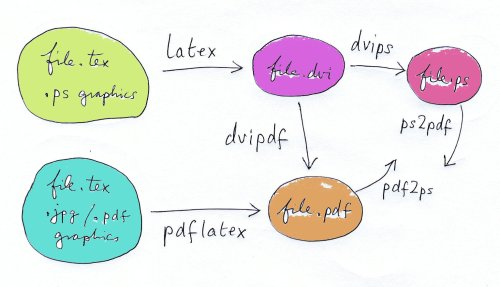
\includegraphics[width=.7\textwidth]{pic1.jpg}
%\includegraphics[width=.7\textwidth]{pic1new.jpg}
\end{center}
It shows the normal routes from a source (\texttt{.tex} file) to
\texttt{.ps} or \texttt{.pdf} output. \textit{Confusion over these
routes is a frequent source of grief}.
\par
It's simplest to keep your image files in the same directory as your
\texttt{.tex} files. Otherwise you can explore the mysteries of
\verb+\graphicspath+ \cite[Sec.~10.2.5]{MG}. In any case, use only
forward slashes in a directory specification. Names of directories and
of graphics files \textit{must not} include spaces!
%
\section{Fancy}
Some text.
\par
\begin{figure}[ht]\centering
  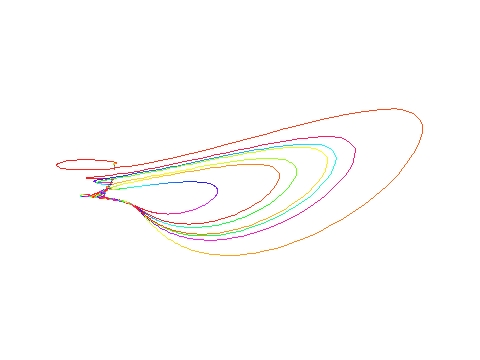
\includegraphics[width=.7\textwidth]{pic3.jpg}
  \caption{This is a caption explaining the diagram
clearly and fully.}\label{fig:pic}
\end{figure}
That is, a picture \lq floating\rq\ in a \texttt{figure} environment
--- with a caption and number as in Fig.~\ref{fig:pic} --- might be
placed by \LaTeX\ on a page well after the text meant to accompany it.
\par
This happens if you have a relatively high density of graphics to
text. You may be able to deal with it by re-distributing the
pictures, changing the size of some of them, and the careful use of
paragraph breaks. Otherwise you may resort to \verb+\clearpage+,
which forces insertion of floating objects waiting to go in.
\par
The \nss\ book \cite{NSS} has Sec.~2.12 on the issue of \lq floating
bodies\rq\ and \comp\ has a whole chapter \cite[Chap.~6]{MG} on \lq
mastering floats'.
\par
Note that inside a \verb+figure+ (or \verb+table+) environment the
\verb+\label+ must always {\em follow} the \verb+\caption+ --- see
\cite[p.~67]{MG}.
\par
\begin{figure}[ht]\centering
\begin{minipage}[c]{.45\textwidth}\centering
  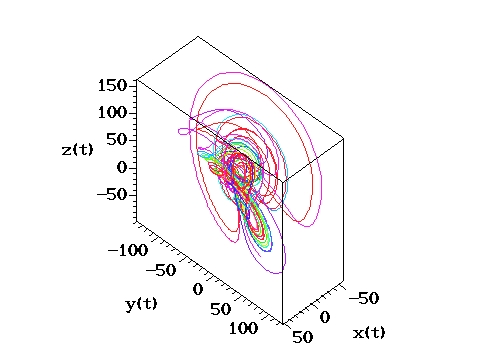
\includegraphics[width=.95\textwidth]{pic4.jpg}
  \caption{Caption to explain the diagram
clearly and fully.}\label{fig:pictwo}
\end{minipage}\hfill
\begin{minipage}[c]{.45\textwidth}\centering
  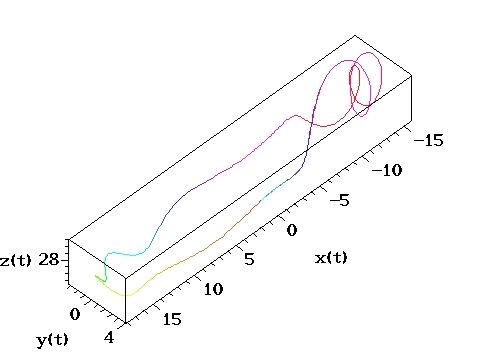
\includegraphics[width=.95\textwidth]{pic5.jpg}\\
  \caption{Caption to explain the diagram
clearly and fully.}\label{fig:picthree}
\end{minipage}
\end{figure}
Fig~\ref{fig:pictwo} and Fig.~\ref{fig:picthree} are two pictures
floating side-by-side, each in a \texttt{minipage} and each with its
own caption and label. This can be an economical way to insert multiple
diagrams.
%
\section{Tables}\label{sec:tables}
Besides figures you may want to include tables. Like figures, tables may
be plain and simple --- short and for immediate and local use only ---
and so put in place without a caption or label; or they may be
complicated and important enough to need a reference label and an
explanatory caption. Here are examples of each in turn.
\par
First a simple table \dots
\par
\begin{center}
 \begin{tabular}{|l||c|c|c|r|}
    \hline
    row 1& it's & just & as & easy \\ \hline
    row 2& as & this & \(E=mc^2\) & what \\ \hline
    row 3& could & be & simpler & ? \\ \hline
    row 4& as & easy & as & \(\Pi\) \\ \hline
  \end{tabular}
\end{center}
\par
Here it is again, now floating in a \texttt{table} environment, with
a caption and a label to identify it as Table~\ref{table:one}.
\begin{table}[h]
  \centering
\begin{tabular}{|l||c|c|c|r|}
    \hline
    row 1& it's & just & as & easy \\ \hline
    row 2& as & this & \(E=mc^2\) & what \\ \hline
    row 3& could & be & simpler & ? \\ \hline
    row 4& as & easy & as & \(\Pi\) \\ \hline
  \end{tabular}
  \caption{Floating table, with a caption to explain it
clearly and fully.}\label{table:one}
\end{table}
%---------
\section{Summary}
Graphics files are evidently straightforward to include. If you need
to go beyond the basics, then refer to \Quote{The Graphics Companion}
\cite{GRM}.
\par
Tables are easy to use too, but don't misuse them. Lengthy data-sets can
be supplied separately on CDrom. Put only summaries in the report,
perhaps as an Appendix.
